\section{Keypoints Detector and Descriptor}

The algorithms that we implemented are based on the ORB to detect and SIFT to describe keypoints, it has slightly modification that were done based on experimental results and requested task.

\subsection{Keypoints Detector} 
We used ORB like interest point detector: the original approach uses FAST(Features from Accelerated Segment Test) to detect interests points and assigns an orientation based in the intensity centroid. 

Originally, FAST uses non-maximum suppression for removing adjacent corners and machine learning to improve the performance of the algorithm. In our implementation we do not use machine learning because the explanation is not clear. Our implementation consider three parameters : 

\begin{itemize}
	\item \textit{Threshold}: this parameter define if each of the sixteen neighbor points is lighter, darker or similar to reference point.
	\item \textit{N} : condition to determine if a point is a keypoint(at least N consecutive neighbors must be lighter or darker to reference point).
	\item \textit{Non-Maximum Suppression}: this parameter signals when remove adjacent corners that are too close between them.
\end{itemize}

FAST does not produce a measure of cornerness (it has large responses along edges). As similar to the original implementation of ORB we employ a Harris corner measure to order and select $P$ keypoints. Another limitation of FAST is that it does not produce orientation. To compensate this issue we use a approach similar to SIFT(ORB use moments of the patch around the keypoint). This technique take a window around of each keypoint and collect gradient directions and magnitudes. Then, a histogram is created for this and the amount added to the bin of the histogram is proportional to the magnitude of gradient at each points. Also, we used a gaussian weighting function, this function is multiplied by the magnitude. The farther away, the lesser the magnitude weight.

Figure~\ref{fig:keypoints} shows results with different parameter settings.

\begin{figure}[h!]
\centering
\begin{subfigure}{0.5\textwidth}
  \centering
  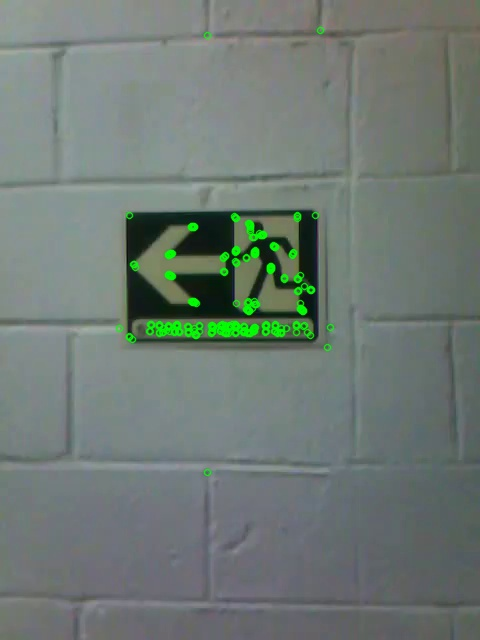
\includegraphics[width=0.5\linewidth]{figs/20-8-false-987.jpg}
  \caption{(20, 8, False). 987 keypoints detected}
\end{subfigure}%
\begin{subfigure}{0.5\textwidth}
  \centering
  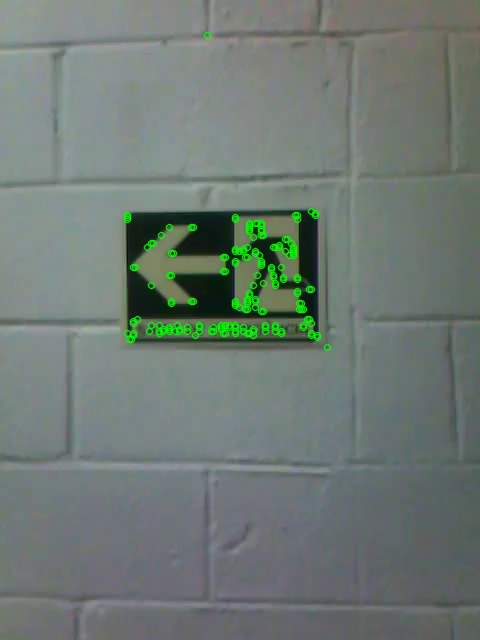
\includegraphics[width=0.5\linewidth]{figs/20-8-true-185.jpg}
  \caption{(20, 8, True). 185 keypoints detected}
\end{subfigure}
\begin{subfigure}{0.5\textwidth}
  \centering
  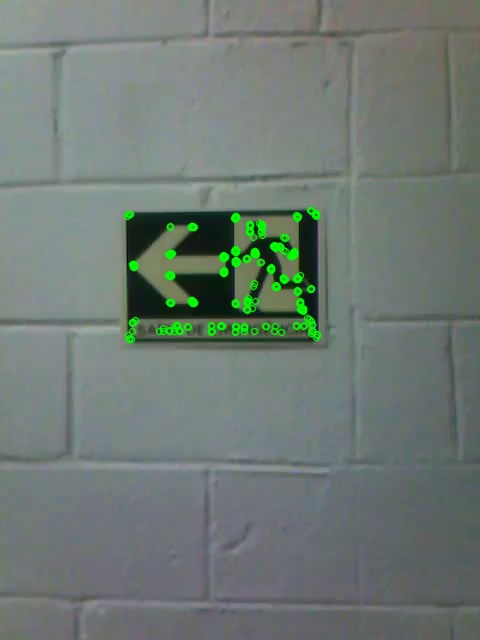
\includegraphics[width=0.5\linewidth]{figs/30-8-false-328.jpg}
  \caption{(30, 8, False). 328 keypoints detected}
\end{subfigure}%
\begin{subfigure}{0.5\textwidth}
  \centering
  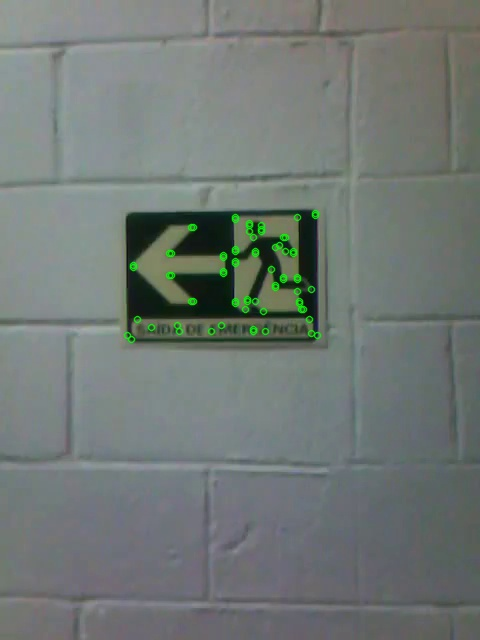
\includegraphics[width=0.5\linewidth]{figs/30-8-true-68.jpg}
  \caption{(30, 8, True). 68 keypoints detected}
\end{subfigure}
\begin{subfigure}{0.5\textwidth}
  \centering
  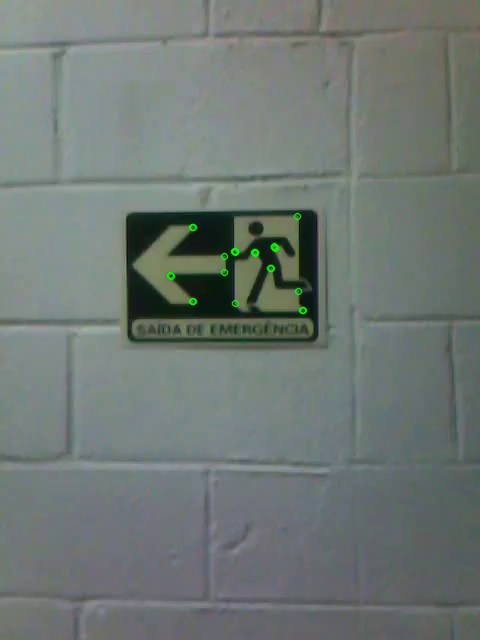
\includegraphics[width=0.5\linewidth]{figs/40-9-false-24.jpg}
  \caption{(40, 9, False). 24 keypoints detected}
\end{subfigure}%
\begin{subfigure}{0.5\textwidth}
  \centering
  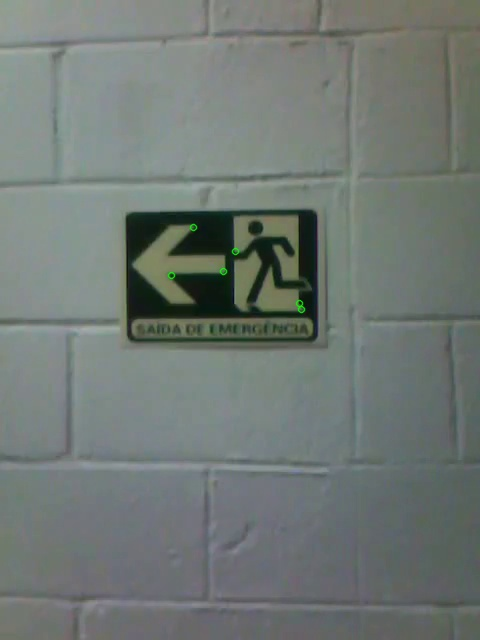
\includegraphics[width=0.5\linewidth]{figs/40-9-true-5.jpg}
  \caption{(40, 9, True). 6 keypoints detected}
\end{subfigure}
 \caption{Results of experiment with different parameter settings. The label of each subfigure follows the following format: \textit{(threshold, N, Non-maximum suppression)} and the number of keypoints detected.}
\label{fig:keypoints}
\end{figure}

According to figure~\ref{fig:keypoints} we can see that with parameter \textit{threshold}, the number of keypoints grows inversely proportional to its value. If we choose a too low value, we start getting false positives and with a too big value, we start ignoring keypoints. This same effect occurs with the parameter $N$.

In the case of \textit{No-Maximal Suppression}, it removes close keypoints, but we have found that this redundancy of keypoints is util for stabilization.


\subsection{Keypoints Descriptor}

The original SIFT considers a pyramid in order to be invariant to scale, the keypoint descriptor is then computed from a specific level of this pyramid. Analysing the data it is easy to see that the scale difference between adjacent frame is negligibly. Thus, our implementation ignores this stage in order to improve the performance of the algorithm.

Figure~\ref{fig:keypoints-match} shows results of the implementation.

\begin{figure}[h!]
\centering
\begin{subfigure}{0.5\textwidth}
  \centering
  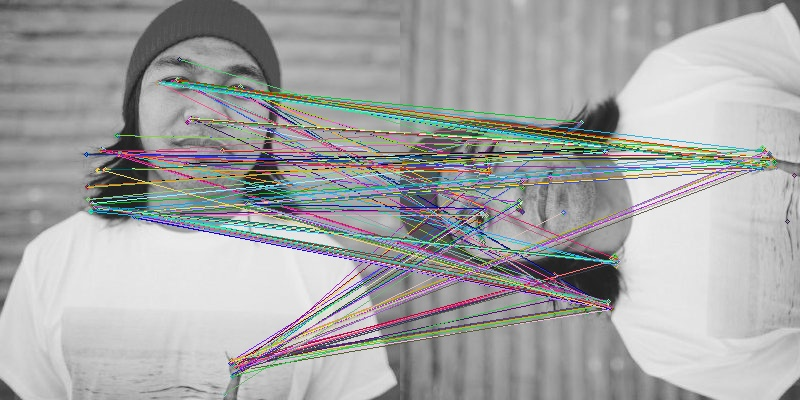
\includegraphics[width=0.9\linewidth]{figs/match-20-8-false.jpg}
  \caption{(20, 8, False).}
\end{subfigure}%
\begin{subfigure}{0.5\textwidth}
  \centering
  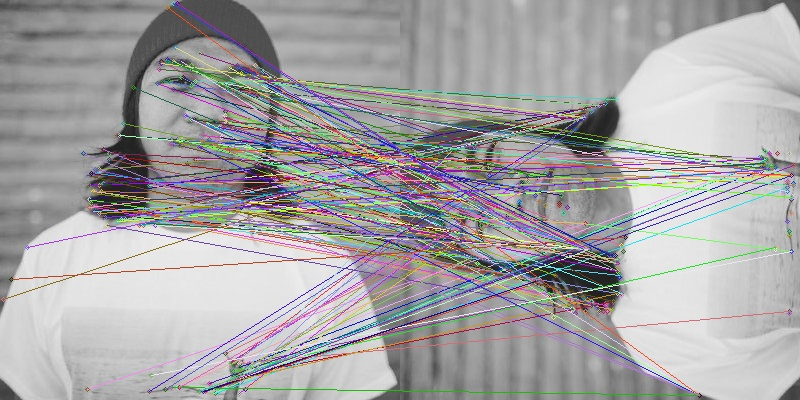
\includegraphics[width=0.9\linewidth]{figs/match-20-8-true.jpg}
  \caption{(20, 8, True).}
\end{subfigure}
\begin{subfigure}{0.5\textwidth}
  \centering
  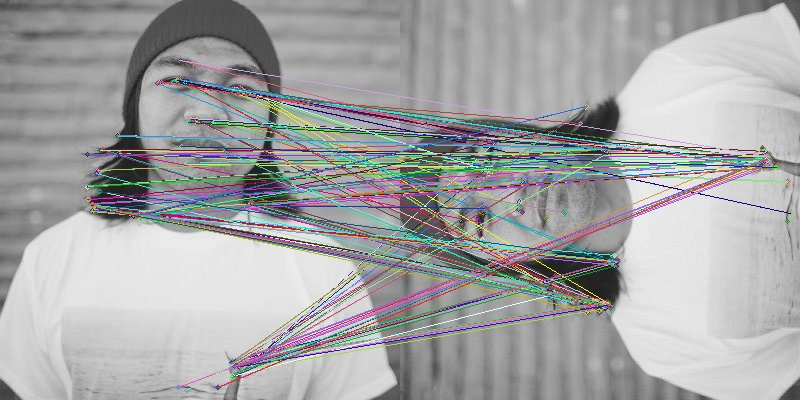
\includegraphics[width=0.9\linewidth]{figs/match-30-8-false.jpg}
  \caption{(30, 8, False).}
\end{subfigure}%
\begin{subfigure}{0.5\textwidth}
  \centering
  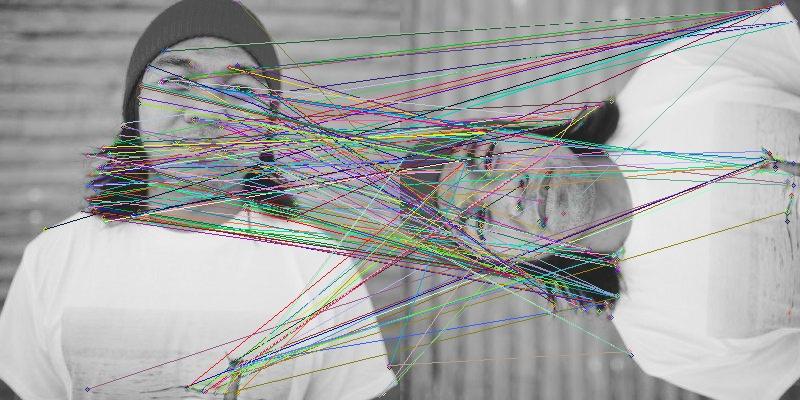
\includegraphics[width=0.9\linewidth]{figs/match-30-8-true.jpg}
  \caption{(30, 8, True).}
\end{subfigure}
\begin{subfigure}{0.5\textwidth}
  \centering
  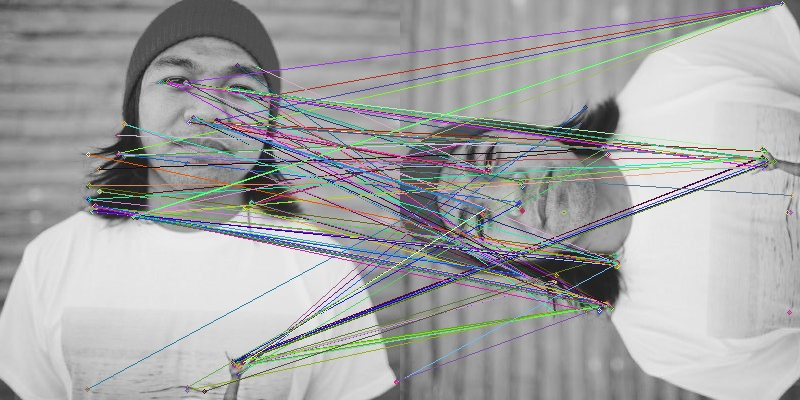
\includegraphics[width=0.9\linewidth]{figs/match-40-9-false.jpg}
  \caption{(40, 9, False).}
\end{subfigure}%
\begin{subfigure}{0.5\textwidth}
  \centering
  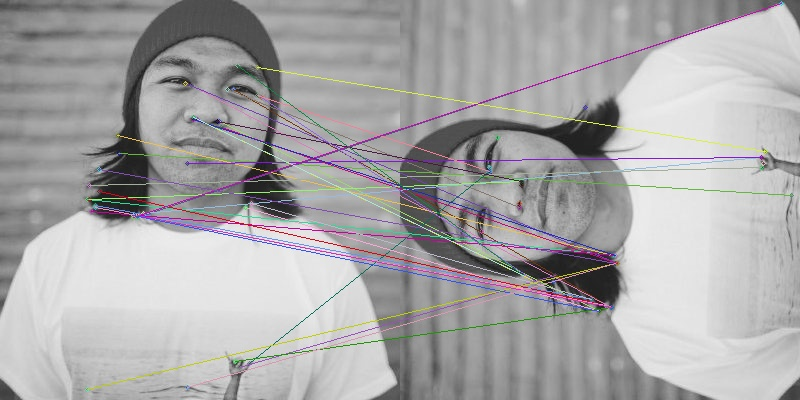
\includegraphics[width=0.9\linewidth]{figs/match-40-9-true.jpg}
  \caption{(40, 9, True).}
\end{subfigure}
 \caption{Results of matches with different parameter settings. The label of each subfigure follows the following format: \textit{(threshold, N, Non-maximum suppression)}}
\label{fig:keypoints-match}
\end{figure}

We can see in figure ~\ref{fig:keypoints-match} that the use of Non-Maximum Suppression create more outlier(wrong matches), this is because removing points that are close to one that will be correctly match decrease the number of inliers.


Our experiments suggest to use a setting of (30,8,False). 

